\documentclass[xcolor={dvipsnames},aspectratio=169,10pt]{beamer}
\usetheme{mx}
\usepackage{graphicx}
\graphicspath{{../../figures}}
%% utility packages
\usepackage{etoolbox}
\usepackage{multicol}
\usepackage{relsize}
\usepackage{fontawesome}

% better text justifying
\usepackage{microtype}
% justify text inside list environment
% Ref: http://liam0205.me/2017/04/11/justifying-in-beamer-s-lists/
\usepackage{ragged2e}
\makeatletter
\patchcmd{\itemize}{\raggedright}{\justifying}{}{}
\patchcmd{\beamer@enum@}{\raggedright}{\justifying}{}{}
\patchcmd{\@@description}{\raggedright}{\justifying}{}{}
\makeatother

% table of content with numbers and justification
% https://tex.stackexchange.com/questions/188773
\setbeamertemplate{section in toc}{\hspace*{1em}\inserttocsectionnumber.~\inserttocsection\par}
\setbeamertemplate{subsection in toc}{\hspace*{2em}\inserttocsectionnumber.\inserttocsubsectionnumber.~\inserttocsubsection\par}

% math related packages
\usepackage{amsmath}
\usepackage[ruled,vlined]{algorithm2e}
\SetAlCapNameFnt{\scriptsize}
\SetAlCapFnt{\scriptsize}
\SetAlFnt{\scriptsize}

% figure related packages
\usepackage{graphicx}
\usepackage[scale=2]{ccicons}
\usepackage{qrcode}
\usepackage{tikz}
\usepackage{tikzpagenodes}
\usetikzlibrary{positioning}

% table related packages
\usepackage{array}
\usepackage{booktabs}
\usepackage{multirow}
\usepackage{colortbl}
\newcommand{\tabincell}[2]{\begin{tabular}{@{}#1@{}}#2\end{tabular}}

% code highlight
\usepackage{listings}
%\usepackage{minted}
%\definecolor{mintedbg}{HTML}{E5E9F0}
%\setminted{autogobble,bgcolor=mintedbg,fontsize=\small}
%\setmintedinline{bgcolor=mintedbg,fontsize=\smaller}
%\newminted{bash}{}
%\newminted{latex}{}
%\newmintinline{bash}{}
%\newmintinline{latex}{}
%\newcommand{\texdoc}[2]{\href{#2}{\bashinline|texdoc #1|}}

% hyperref setting
\hypersetup{
  unicode,
  psdextra,
  bookmarksnumbered=true,
  bookmarksopen=true,
  bookmarksopenlevel=3,
  bookmarksdepth=4,
  pdfcenterwindow=true,
  pdfstartview={Fit},
  pdfpagemode={FullScreen},
  pdfpagelayout={SinglePage},
}
\usepackage{bookmark}

% beamer theme
\usetheme{metropolis}
\metroset{block=fill,numbering=fraction}

% caption style
\usepackage{subcaption}
\setlength\abovecaptionskip{3pt}
\setbeamerfont{caption}{size=\scriptsize}
\renewcommand{\figurename}{Fig.}
\captionsetup{labelformat=empty,labelsep=none,textfont={bf,it}}

% Ref: https://github.com/gpoore/minted/blob/master/source/minted.dtx
\newenvironment{latexexample}
{\VerbatimEnvironment\begin{VerbatimOut}[gobble=3]{example.out}}{\end{VerbatimOut}%
  \begin{center}
    \begin{minipage}{0.47\linewidth}%
      \inputminted[resetmargins,fontsize=\scriptsize]{latex}{example.out}%
    \end{minipage}%
    \hspace{0.05\linewidth}%
    \begin{minipage}{0.47\linewidth}%
      \begin{framed}
        \setlength{\parindent}{2em}%
        \input{example.out}%
      \end{framed}
    \end{minipage}%
  \end{center}
}

\newenvironment{mathexample}
{\VerbatimEnvironment\begin{VerbatimOut}[gobble=3]{example.out}}{\end{VerbatimOut}%
  \begin{center}
    \begin{minipage}{0.47\linewidth}%
      \inputminted[resetmargins,fontsize=\scriptsize]{latex}{example.out}%
    \end{minipage}%
    \hspace{0.05\linewidth}%
    \begin{minipage}{0.47\linewidth}%
      \begin{framed}
        \[ \input{example.out} \]
      \end{framed}
    \end{minipage}%
  \end{center}
}

\newenvironment{mathexamples}
{\VerbatimEnvironment\begin{VerbatimOut}[gobble=3]{example.out}}{\end{VerbatimOut}%
  \begin{center}
    \begin{minipage}{0.47\linewidth}%
      \inputminted[resetmargins,fontsize=\scriptsize]{latex}{example.out}%
    \end{minipage}%
    \hspace{0.05\linewidth}%
    \begin{minipage}{0.47\linewidth}%
      \begin{framed}
        \directlua{
          local first = true
          for line in io.lines('example.out') do
          if first then
          first = false
          else
          tex.print('\\newline ')
          end
          tex.print('$' .. line .. '$')
          end
        }
      \end{framed}
    \end{minipage}%
  \end{center}
}



%---------------------------------------------------------------------
% Add Paper using {\paper{}. begin{beawer} ... end{beamer} }
%---------------------------------------------------------------------
\newcommand\paper[1]{
	\setbeamertemplate{footline}
	{
		\begin{beamercolorbox}[wd=\textwidth,ht=3mm,dp=03mm,leftskip=0.3cm,rightskip=0.3cm]{black}%
        		\usebeamerfont{page number in head/foot}
			(#1)\mbox{}\hfill\insertframenumber
		\end{beamercolorbox}%
	}
}



\title{  
Towards lightweight transformer-based models with multimodal data for low-latency surgical applications
}
\subtitle{Fast Machine Learning for Science Workshop 2023}

\author{
Sujon Hekim, Stephen Thompson, and \\
{\bf Miguel Xochicale, PhD} (\faTwitter @\_mxochicale  \faGithub @mxochicale)
}

\date{
September 26, 2023; 17:00 - 17:15
% \today
}

\institute{
	Advanced Research Computing Centre and WEISS \\
	University College London
	}

\titlegraphic{
  \begin{tikzpicture}[overlay, remember picture]
    \node[%
      above right=0.35cm and -0.2cm of current page footer area.south west,
      anchor=south west,
      inner sep=0pt] {%
      \usebeamerfont{footline}
      \begin{tabular}{lm{.8\textwidth}}
        \href{http://creativecommons.org/licenses/by/4.0/}{\ccby} &
        This slices is licensed under a
	\href{http://creativecommons.org/licenses/by/4.0/}
		{Creative Commons ``Attribution 4.0 International''} license. 
	\par Get source of this slides and see further references 
		from \url{https://github.com/mxochicale/rtt4ssa}.
      \end{tabular}
    };
    \node[%
      above left=0.35cm and 0cm of current page footer area.south east,
      anchor=south east,
      inner sep=0pt]{\qrcode[height=1.5cm]{https://github.com/mxochicale/rtt4ssa}};
  \end{tikzpicture}
}

\begin{document}

\maketitle

\begin{frame}
\frametitle{Table of Contents}
    \tableofcontents
\end{frame}


%%%%%%%%%%%%%%%%%%%%%%%%%%%%%%%%%%%%%%%%%%%%
\section{Introduction}

\begin{frame}
  \frametitle{Table of Contents}
  \tableofcontents[currentsection]
\end{frame}



\subsection{Clinical background}

%%%%%%%%%%%%%%%%%%%%%%%%%%%%%%%%%%%%%%%%%%%%%%%%%%%%%%%%
{
\paper{
ZUKETANG-Laparoscope-Laparoscopic-Simulator-Instruments;
Simendo simulator;
Laparo Analytic;
Gustavo A. Alonso-Silverio et al. in Surgical Education: Training for the Future 2018.
}

\begin{frame}{Training Surgical Skills}
      \begin{figure}
        \centering
        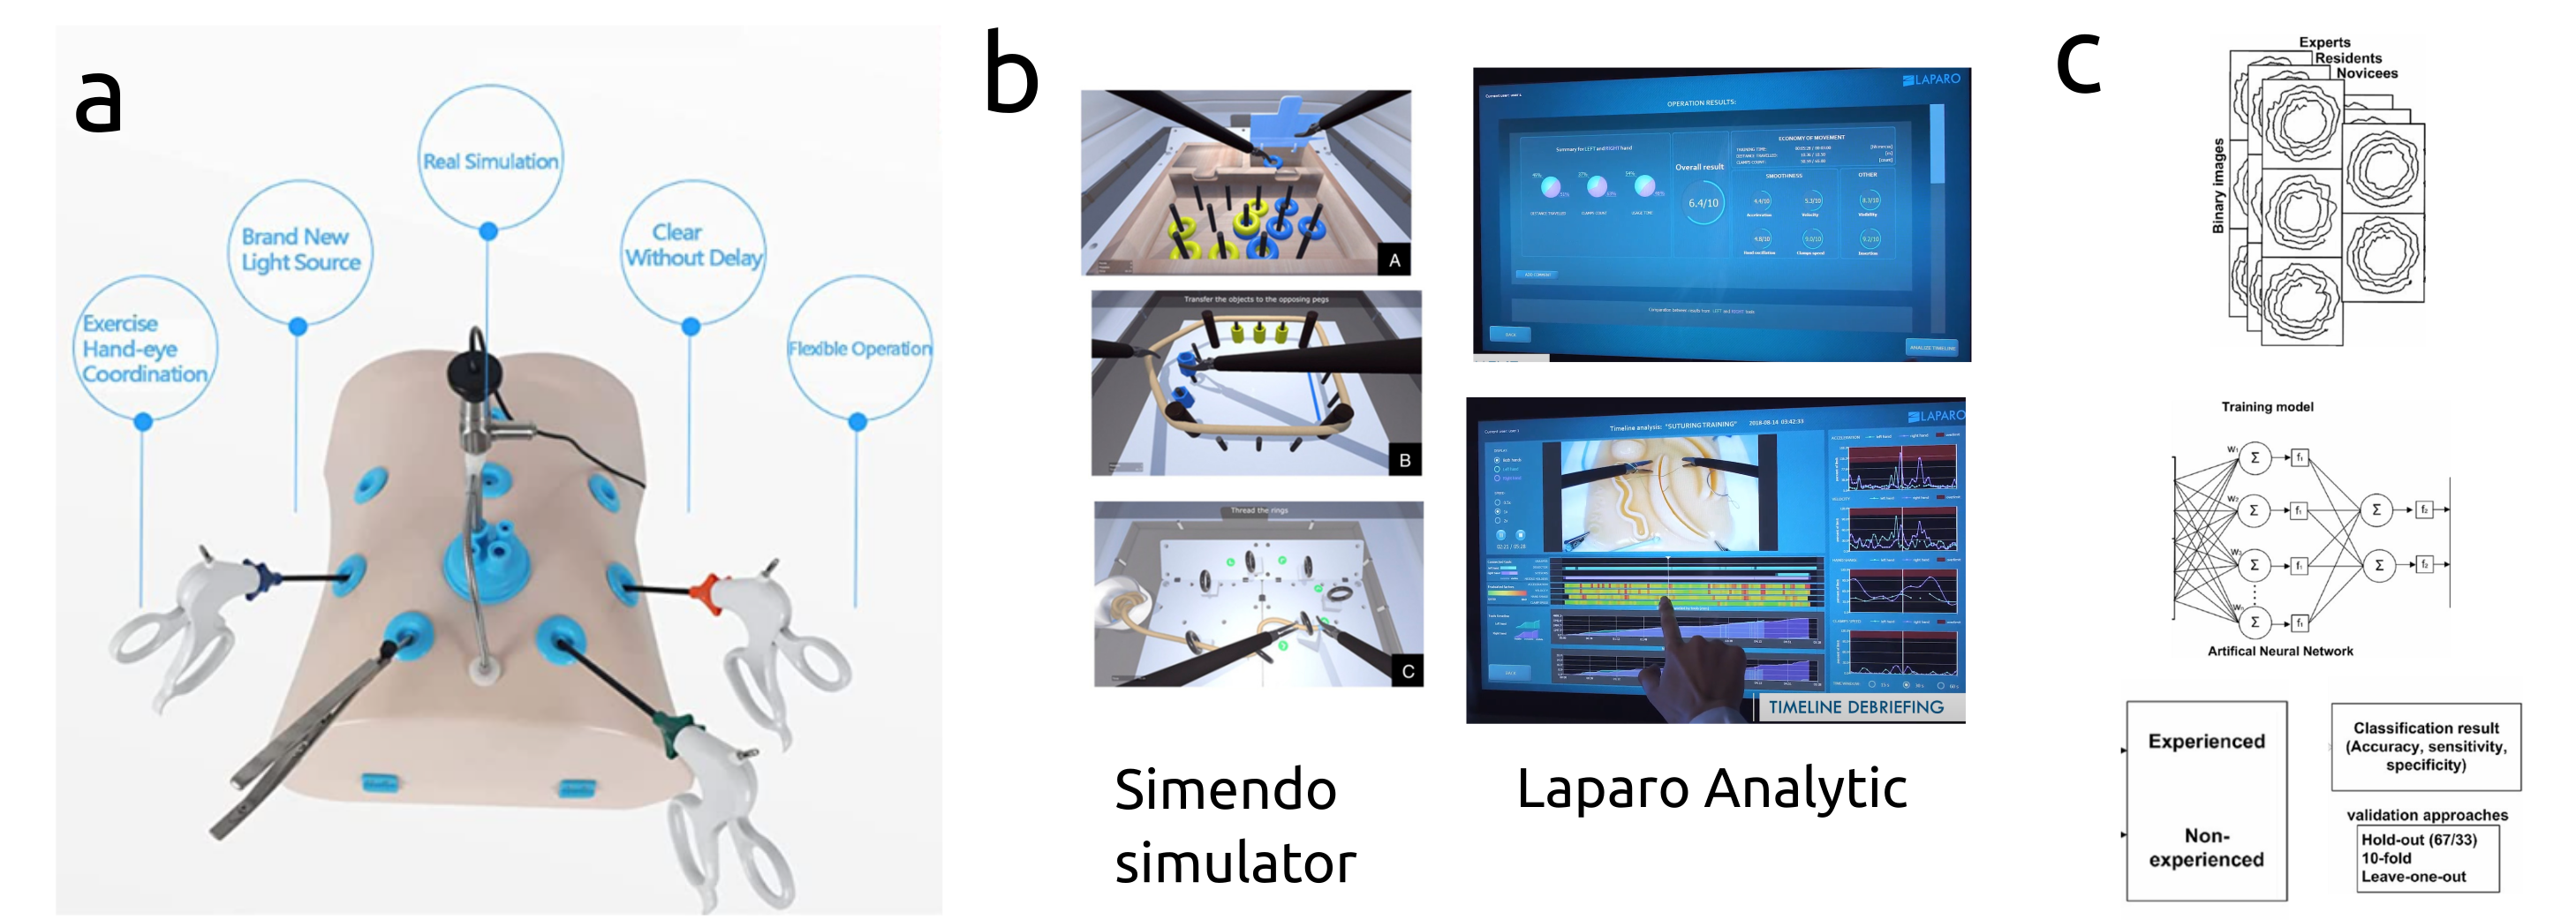
\includegraphics[width=1.0\textwidth]{main/outputs/drawing-v00.png}
        % \caption{The sonographer-probe-patient control system}
      \end{figure}
\end{frame}
}


\subsection{Research aims}
%%%%%%%%%%%%%%%%%%%%%%%%%%%%%%%%%%%%%%%%%%%%%%%%%%%%%%%%
{
%\paper{Wright-Gilbertson M. 2014 in PhD thesis}
\begin{frame}{Research aims}
\begin{itemize}
\item Design of reproducible workflow for data collection using multimodal sensors (e.g., USB video image and Bluetooth-based inertial sensors)
\item Investigate DL models with small memory and parameter size to enhance inference speed for surgical applications
% \item
\end{itemize}

\end{frame}
}


%%%%%%%%%%%%%%%%%%%%%%%%%%%%%%%%%%%%%%%%%%%
\section{Lightweight transformer-based models}

\begin{frame}
      \frametitle{Table of Contents}
      \tableofcontents[currentsection]
\end{frame}

% \subsection{Clinical background}

%%%%%%%%%%%%%%%%%%%%%%%%%%%%%%%%%%%%%%%%%%%%%%%%%%%%%%%%
{
\paper{
Menghani, Gaurav. "Efficient deep learning: A survey on making deep learning models smaller, faster, and better." ACM Computing Surveys 55, no. 12 (2023): 1-37.
% https://dl.acm.org/doi/full/10.1145/3578938
}

\begin{frame}{Efficient deep learning}
      \begin{figure}
        \centering
        
\includegraphics[width=1.0\textwidth]{lightweight-transformer-A/outputs/drawing-v00}
        % \caption{The sonographer-probe-patient control system}
      \end{figure}
\end{frame}
}


%%%%%%%%%%%%%%%%%%%%%%%%%%%%%%%%%%%%%%%%%%%%%%%%%%%%%%%%
{
\paper{
% Li, Yanyu, Ju Hu, Yang Wen, Georgios Evangelidis, Kamyar Salahi, Yanzhi Wang, Sergey Tulyakov, and Jian Ren. "Rethinking vision transformers for mobilenet size and speed." arXiv preprint arXiv:2212.08059 (2022).
(a) Li et al. "Rethinking vision transformers for mobilenet size and speed." arXiv preprint arXiv:2212.08059 (2022).

% EfficientFormerV2 Dec-2022 https://arxiv.org/abs/2212.08059 > https://github.com/snap-research/EfficientFormer
% Zhang, Wenqiang, Zilong Huang, Guozhong Luo, Tao Chen, Xinggang Wang, Wenyu Liu, Gang Yu, and Chunhua Shen. "TopFormer: Token pyramid transformer for mobile semantic segmentation." In Proceedings of the IEEE/CVF Conference on Computer Vision and Pattern Recognition, pp. 12083-12093. 2022.
(b) Zhang et al. "TopFormer: Token pyramid transformer for mobile semantic segmentation." In Proceedings of the IEEE/CVF Conference on Computer Vision and Pattern Recognition, pp. 12083-12093. 2022.
% Topformer Apr-2022 https://arxiv.org/abs/2204.05525 > https://github.com/hustvl/TopFormer
}


\begin{frame}{Lightweight transformer-based models}
      \begin{figure}
        \centering
        
\includegraphics[width=1.0\textwidth]{lightweight-transformer-B/outputs/drawing-v00}
        % \caption{The sonographer-probe-patient control system}
      \end{figure}
\end{frame}
}


%OTHER RELEVANT REFERENCES
% CFPNet-M: A Light-Weight Encoder-Decoder
% Based Network for Multimodal Biomedical Image
% Real-Time Segmentation
%
% The
% CFPNet-M achieves segmentation results on all five
% medical datasets that are comparable to existing methods,
% yet require only 8.8 MB memory, and just 0.65 million
% parameters, which is about 2% of U-Net. Unlike other deep-
% learning segmentation methods, this new approach is
% suitable for real-time application: its inference speed can
% reach 80 frames per second when implemented on a single
% RTX 2070Ti GPU with an input image size of 256×192 pixels.


% Papa, Lorenzo, Paolo Russo, Irene Amerini, and Luping Zhou. "A survey on efficient vision transformers: algorithms, techniques, and performance benchmarking." arXiv preprint arXiv:2309.02031 (2023).
% https://arxiv.org/abs/2309.02031



%%%%%%%%%%%%%%%%%%%%%%%%%%%%%%%%%%%%%%%%%%%%
\section{Experiments and demo datasets}

\begin{frame}
      \frametitle{Table of Contents}
      \tableofcontents[currentsection]
\end{frame}

% \subsection{Clinical background}

%%%%%%%%%%%%%%%%%%%%%%%%%%%%%%%%%%%%%%%%%%%%%%%%%%%%%%%%
{
\paper{
Khogali-Jakary et al., in Surgical Endoscopy (2020)
}

\begin{frame}{Data collection}
      \begin{figure}
        \centering
        
\includegraphics[width=1.0\textwidth]{experiments-24-aug-2023-B/outputs/drawing-v00}
        % \caption{The sonographer-probe-patient control system}
      \end{figure}
\end{frame}
}

%%%%%%%%%%%%%%%%%%%%%%%%%%%%%%%%%%%%%%%%%%%%%%%%%%%%%%%%
{
\paper{
Haralick, RM.; Shanmugam, K., "Textural features for image classification" in IEEE Transactions on systems, man, and cybernetics 6 (1973): 610-621.
%GLCM >  https://youtu.be/wYZzpE1pPn0?feature=shared&t=784
% National-Health-Service 2021. Screening for down’s syndrome, edwards’ syndrome and patau’s syndrome. \url{https://www.nhs.uk/pregnancy/your-pregnancy-care}
}

\begin{frame}{Multimodal data}{Video[3-channels; 480Hx650W] and motion time-series data}
      \begin{figure}
        \centering
        
\includegraphics[width=1.0\textwidth]{experiments-24-aug-2023-A/outputs/drawing-v00}
        % \caption{The sonographer-probe-patient control system}
      \end{figure}
\end{frame}
}




%%%%%%%%%%%%%%%%%%%%%%%%%%%%%%%%%%%%%%%%%%%%
\section{Preliminary Results}

\begin{frame}
      \frametitle{Table of Contents}
      \tableofcontents[currentsection]
\end{frame}

% \subsection{Clinical background}

%%%%%%%%%%%%%%%%%%%%%%%%%%%%%%%%%%%%%%%%%%%%%%%%%%%%%%%%
{
\paper{
\url{https://keras.io/examples/timeseries/timeseries_classification_from_scratch} by hfawaz
}

\begin{frame}{Timeseries classification with CNN model}
      \begin{figure}
        \centering
        
\includegraphics[width=1.0\textwidth]{results-timeseries_classification_from_scratch-24-aug-2023/outputs/drawing-v00}
        % \caption{The sonographer-probe-patient control system}
      \end{figure}
\end{frame}
}


%%%%%%%%%%%%%%%%%%%%%%%%%%%%%%%%%%%%%%%%%%%%%%%%%%%%%%%%
{
\paper{
\url{https://keras.io/examples/timeseries/timeseries_classification_transformer/} by Theodoros Ntakouris
}

\begin{frame}{Timeseries classification with a Transformer model}
      \begin{figure}
        \centering
        
\includegraphics[width=1.0\textwidth]{results-timeseries_classification_transformer-24-aug-2023/outputs/drawing-v00}
        % \caption{The sonographer-probe-patient control system}
      \end{figure}
\end{frame}
}


%%%%%%%%%%%%%%%%%%%%%%%%%%%%%%%%%%%%%%%%%%%%
\section{Conclusions and future work}

\begin{frame}
  \frametitle{Table of Contents}
  \tableofcontents[currentsection]
\end{frame}

\subsection{Conclusions}
%%%%%%%%%%%%%%%%%%%%%%%%%%%%%%%%%%%%%%%%%%%%%%%%%%%%%%%%
{
\paper{
Sciortino et al. in Computers in Biology and Medicine 2017 https://doi.org/10.1016/j.compbiomed.2017.01.008;
He et al. in Front. Med. 2021 https://doi.org/10.3389/fmed.2021.729978
}
\begin{frame}{Conclusions}

\begin{itemize}
\item Proposed a data-collection protocol for video and tracking data
\item Prototyped CNN and transformer based models for time-series classification of multimodal data
\end{itemize}

\end{frame}
}


\subsection{Future work}
%%%%%%%%%%%%%%%%%%%%%%%%%%%%%%%%%%%%%%%%%%%%%%%%%%%%%%%%
{
\paper{
Menghani, Gaurav. "Efficient deep learning: A survey on making deep learning models smaller, faster, and better." ACM Computing Surveys 55, no. 12 (2023): 1-37.
}
\begin{frame}{Future work}

\begin{itemize}
\item Benchmarks for fficient architectures \\ (cheaper training for large models and inference costs)
\item Dedicated hardware for specialized use cases (fpga-dev-kit)
\item Contribute to open public datasets
\end{itemize}

\end{frame}
}


%%%%%%%%%%%%%%%%%%%%%%%%%%%%%%%%%%%%%%%%%%%%
\subsection{GitHub repository}

%%%%%%%%%%%%%%%%%%%%%%%%%%%%%%%%%%%%%%%%%%%%%%%%%%%%%%%%
{
\paper{
GitHub repository \url{https://github.com/mxochicale/rtt4ssa}
}
\begin{frame}{GitHub repository: rtt4ssa}
Real-time transformer-based models for surgical skills assessment

      \begin{figure}
        \centering
        
\includegraphics[width=1.0\textwidth]{github_repo_rtt4ssa/outputs/drawing-v00}
      \end{figure}

\end{frame}
}


% \maketitle

\end{document}

